\documentclass{mipt-thesis-bs}
\usepackage{listings}
\usepackage{biblatex}
\addbibresource{thesis.bib}
\title{Разработка методов отладки в реальном времени и отложенного анализа проблем в гостевой операционной системе Microsoft Windows под гипервизором QEMU/KVM}
\author{Прутьянов В.\,В.}
\supervisor{Каган Р.\,В.}
\groupnum{416}
\faculty{Факультет радиотехники и кибернетики}
\department{Кафедра теоретической и прикладной информатики}

\begin{document}
\titlecontents

\chapter{Введение}

В настоящее время большая часть рабочей серверной нагрузки выполняется с помощью различных технологий виртуализации. Виртуализация позволяет на основе одной физической системы запускать множество независимых друг от друга изолированных сред, между которыми могут быть распределены вычислительные ресурсы физической системы.

Одним из видов виртуализации является гипервизорная виртуализация. В этом случае, специальное ПО, называемое гипервизором, который может быть как частью операционной системы, так и непосредственно выполняться на физическом оборудовании, позволяет разделить физические ресурсы между изолированными средами, которые называются виртуальными машинами. Тогда физическое оборудование, на котором запущен гипервизор называется хостом, а виртуальные машины называются гостями.

Сейчас в качестве хостовой ОС на серверах часто используется ОС Linux. Один из компонентов этой системы -- гипервизор KVM, который работает в связке с эмулятором QEMU. Операционные системы, работающие внутри хоста и гостей, могут быть различными в случае гипервизорной виртуализации, поэтому внутри виртуальной машины под управлением QEMU/KVM может быть запущена почти любая ОС, в том числе Linux и Microsoft Windows.

Виртуализация, в частности гипервизорная, является достаточно сложной процедурой, поэтому при работе гостевой ОС могут возникать проблемы, такие как зависания или аварийные завершения. Эти проблемы могут быть вызваны как ошибками в работе гостевой ОС, так и ошибками, связанными с неправильной работой гипервизора. Существуют два метода выяснения причин подобных проблем: отладка ядра гостевой ОС и анализ снимков состояния виртуальной машины, называемых дампами.

Для гостевой Linux оба метода удобны и не представляют большой сложности при работе с QEMU:

\begin{itemize}
\item QEMU предоставляет интерфейс для отладчика GDB, через который можно отлаживать ядро гостевой ОС Linux как обычную программу.
\item QEMU позволяет сделать снимок состояния виртуальной машины, называемый дампом , в формате ELF, который затем можно анализировать утилитой crash
\end{itemize}

Аналоги этих методов существуют и для случая, когда виртуальная машина работает под управлением Windows:

\begin{itemize}
\item Подключение через виртуальный последовательный порт или Ethernet отладчика WinDbg
\item Создание отладочного дампа в формате DMP, понятном отладчику WinDbg, и его анализ.
\end{itemize}

Поскольку, как правило, администрируют хостовые системы и гостевые системы разные люди, наиболее предпочтительным для любой гостевой ОС является создание отладочных дампов, так как это требует наименьшее количество действий (или вовсе не требует) от пользователя виртуальной машины, который может не обладать желанием или соответствующей квалификацией для настройки гостевой ОС в режиме отладки. Также, метод создания и анализа отладочных дампов не требует специального воспроизведения условий, приводящих к ошибке. Таким образом, возможность снятия отладочных дампов имеет наибольшую ценность для разработчиков ПО виртуализации.

На данный момент метод, связанный с анализом дампов, в случае гостевой ОС Windows под управлением QEMU имеет существенные проблемы:

\begin{itemize}
\item QEMU не имеет встроенного средства для создания дампов памяти в формате DMP. Для получения дампа в этом формате в произвольный момент времени на живой системе можно попытаться создать дамп в формате ELF и конвертировать его в формат DMP, но это не всегда возможно, особенно на последних версиях Windows.
\item В случае аварийного завершения Windows автоматически сохраняет дамп на диске, что сопровождается так называемым BSoD (англ. Blue Screen of Death - синий экран смерти), но для этого, во-первых, система должна быть настроена на создание полного дампа памяти, который наиболее полно отражает состояние системы (по умолчанию же сохраняется практически бесполезный малый дамп памяти), а во-вторых, дамп может быть не создан, например, если не хватает свободного места на диске, или по другим причинам\cite{nodump}.
\end{itemize}

Таким образом, одним из важных сценариев является создание дампа в момент возникновения BSoD, когда гостевая система по каким-либо причинам не способна это сделать. Поэтому представляется актуальным разработка метода создания отладочного дампа гостевой Windows в формате, понятном отладчику WinDbg, как в случае живой системы, так и на этапе аварийного завершения.

На данный момент выпущено много различных версии Windows, из которых сейчас действительно популярны серверные системы начиная с Windows Server 2008 R2 и десктопные системы начиная с Windows 7, которые работают на основе одного ядра Windows версии 6.1. Также, наиболее популярными сейчас являются 64-битные версии, поэтому в работе будут рассмотрены 64-битные версии Windows на основе этой версии ядра и старше.

Так как в различных версиях Windows определения структур данных ядра могут различаться, хорошей чертой метода была бы независимость от версии Windows. Это бы означало использование более прозрачной логики и увеличивало бы шансы метода на корректную работу с новыми версиями Windows.

В работе будет рассмотрено, из чего состоит полный дамп памяти Windows, какие данные требуются для его создания, существующие методы их сбора и предложен подход для создания дампа во время BSoD, а также расширение этого подхода для работы на живой системе.

\chapter{Постановка задачи}

\begin{itemize}
\item Исследовать, какие данные необходимы для создания полного дампа памяти и как они могут быть получены.
\item Разработать метод снятия полных дампов памяти в формате DMP с 64-разрядной гостевой ОС Windows с версией ядра $\geqslant$ 6.1, работающей под управлением QEMU/KVM, в момент аварийного завершения.
\item Добавить возможность снятия дампов с живой системы.
\item Программно реализовать эти методы.
\end{itemize}

\chapter{Основные используемые технологии и инструменты}

\section*{QEMU}

QEMU -- эмулятор аппаратного обеспечения с открытым исходным кодом, который позволяет эмулировать x86-совместимый процессор и периферию и запускать на нем соответствующее ПО. Также существует возможность ускорения работы с помощью KVM, Xen, Apple Hypervisor Framework или других ускорителей.

\section*{KVM}

KVM (Kernel-based Virtual Machine) -- технология виртуализации, встроенная в ядро Linux. Для работы использует одну из технологий аппаратной поддержки виртуализации, например, Intel VT-x или AMD-V. Сама по себе не занимается эмуляцией, а только предоставляет интерфейс к возможностям аппаратной виртуализации такому инструменту как QEMU.

\section*{QEMU/KVM}
Одним из наиболее популярных вариантов, в том числе на корпоративном рынке, является связка QEMU/KVM, которая позволяет программному обеспечению внутри виртуальной машины достичь скорости работы близкой к скорости на хостовой машине. В таком режиме работы QEMU не производит эмуляцию инструкций, а делегирует выполнение кода процессору через KVM.

\section*{WinDbg}

WinDbg -- отладчик от корпорации Microsoft для отладки как пользовательского, так и системного кода под ОС Windows. Имеет возможность анализа дампов падений Windows. Вместе с WinDbg распространяется программа dumpchk.exe, которая предназначена для обнаружения ошибок в дампах.

\section*{WDK}

WDK (Windows Driver Kit) -- набор инструментов и библиотек для разработки драйверов под ОС Windows. Кроме того, содержит заголовочные файлы с описаниями некоторых структур ядра Windows.

\chapter{Полный дамп памяти}

В ОС Windows существует несколько различных форматов дампов, набор которых различается в зависимости от версии Windows\cite{dumps}. В данной работе рассматривается полный дамп памяти (англ. complete memory dump), который доступен во всех рассматриваемых версиях Windows. Этот тип дампа содержит наибольшее количество информации и позволяет отладчику анализировать весь объем используемой системой физической памяти\cite{completedump}.

К сожалению, официальной спецификации формата DMP от компании Microsoft не существует. Наиболее полное описание структуры заголовка полного дампа может быть найдено в коде операционной системы Singularity (экспериментальная ОС с открытым исходным кодом от Microsoft)\cite{mssing}, хотя объяснения смысла полей нет и там.

Структура полного дампа (\picref{fig:dmp-scheme}) в упрощенном виде представляет из себя несколько крупных частей:

\begin{itemize}
    \item Заголовок длиной в одну страницу (4 килобайт) на 32-разрядной системе и длиной 2 страницы на 64-разрядной системе.
    \item Снимки непрерывных регионов физической памяти. Их количество, начальные адреса и длины хранятся в заголовке.
\end{itemize}

\begin{figure}[h]
\begin{center}
    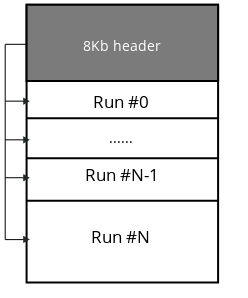
\includegraphics[width=5cm]{dmp_scheme1.png}
    \caption{Упрощенная cхема полного дампа}
    \label{fig:dmp-scheme}
\end{center}
\end{figure}

Информацию о сохраненной в файле дампа физической памяти может отображать утилита dumpchk.exe (\picref{fig:runs}), поставляющаяся в месте с отладчиком WinDbg. Этих регионов больше одного из-за так называемых PCI-окон (англ. PCI-hole), поскольку часть физического адресного пространства используется для коммуникации с периферийными устройствами и не подходит сохранения данных. Таким образом, не все физическое адресное пространство сохраняется в файле дампа.

\begin{figure}[h]
\begin{center}
    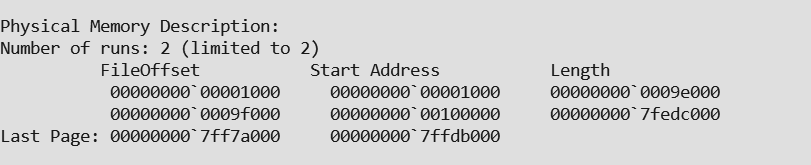
\includegraphics[width=1\textwidth]{runs.png}
    \caption{Список регионов физической памяти отображается утилитой dumpchk.exe}
    \label{fig:runs}
\end{center}
\end{figure}

Каждый регион физической памяти описывается в заголовке дампа структурой {\_}PHYSICAL{\_}MEMORY{\_}RUN64, где хранится начало и длина региона:

\begin{verbatim}
struct _PHYSICAL_MEMORY_RUN64 {
    ULONG64 BasePage;
    ULONG64 PageCount;
}
\end{verbatim}

Кроме информации о регионах физической памяти, заголовок дампа содержит другие необходимые для работы отладчика поля, в том числе:

\begin{itemize}
        \item BugcheckData -- код ошибки и 4 параметра, которые описывают причину аварийного завершения системы. Их можно увидеть на синем экране во время падения (\picref{fig:bsod}). Отладчик WinDbg анализирует эти значения и выводит примерную причину падения (\picref{fig:windbg-analyze}).
    \item RequiredDumpSpace -- суммарный размер дампа в байтах
    \item DirectoryTableBase -- физический адрес начала таблицы страниц, на основе которой отладчик будет производить страничное преобразование для доступа к данным по виртуальным адресам
    \item PfnDatabase -- виртуальный адрес базы данных PFN-номеров\cite{winternals2}
    \item PsLoadedModuleList -- виртуальный адрес списка загруженных исполняемых модулей
    \item KdDebuggerDataBlock -- виртуальный адрес специальной структуры ядра Windows, хранящей необходимую для работы отладчика информацию.
    \item MinorVersion, MajorVersion - два поля, вместе определяющие версию Windows
\end{itemize}

\begin{figure}[h]
\begin{center}
    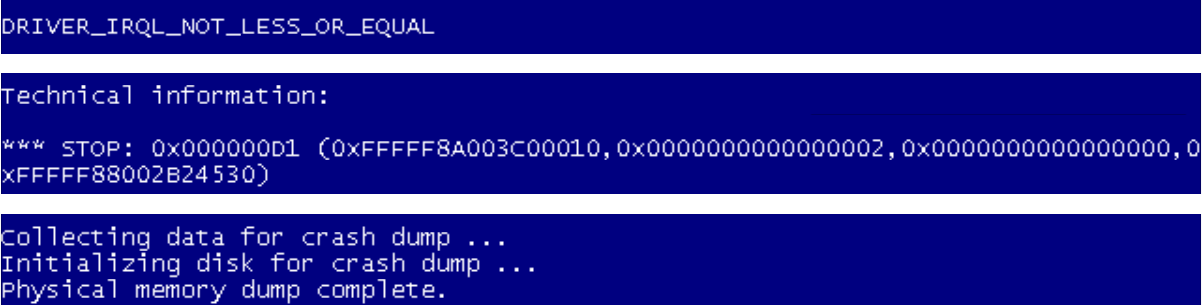
\includegraphics[width=1\textwidth]{dump.png}
    \caption{Фрагменты BSoD}
    \label{fig:bsod}
\end{center}
\end{figure}

\begin{figure}[h]
\begin{center}
    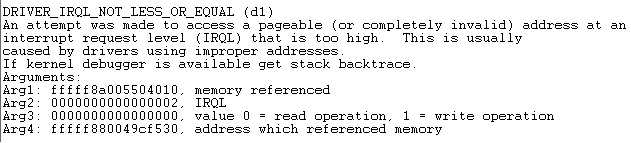
\includegraphics{ss1.png}
    \caption{Bugcheck-анализ в WinDbg}
    \label{fig:windbg-analyze}
\end{center}
\end{figure}

Структура KdDebuggerDataBlock содержит адреса других важные структуры данных ядра и смещения внутри них, например:
\begin{itemize}
\item KernBase -- виртуальный адрес загруженного в память образа ядра Windows (ntoskrnl.exe), используется для загрузки подходящих отладочных символов
\item KiProcessorBlock -- указатель на массив указателей на PRCB (processor control block) -- структуры, в которые ОС сохраняет данные по каждому используемому процессору\cite{winternals1}.
\item OffsetPrcbContext -- в соответствии с названием, смещение структуры внутри PRCB, в которую ОС сохраняет регистровый контекст при аварийном завершении.
\item KiBugcheckData -- указатель на данные о падении, которые автоматически сохраняются в это поле системой во время аварийного завершения. По сути, дублирует поле с похожим названием из заголовка.
\end{itemize}

BugcheckData это не единственно поле, которое присутствует и в структуре заголовка и в структуре KdDebuggerDataBlock.

В отличие от заголовка дампа, структуру содержимого KdDebuggerDataBlock можно увидеть в файле wdbgexts.h, который поставляется вместе с WinDbg. Эта структура обладает таким свойством, что с появлением новой версии Windows в ее конец только добавляются новые поля, а уже существующие остаются по тем же смещениям, на это можно полагаться независимо от версии Windows.

Можно заметить, что если такие поля заголовка как RequiredDumpSpace при определенных условиях можно вычислить и заполнить на основе данных из гипервизора, то такие поля как KdDebuggerDataBlock и PsLoadedModuleList известны только гостевой ОС.

Таким образом, для получения правильного дампа, нужно собрать вместе корректный заголовок и снимки непрерывных участков физической памяти. Снимки несложно сделать из QEMU, поскольку он имеет удобный доступ к физической памяти виртуальной машины. Получение же заголовка, как можно было понять из описания его полей, является нетривиальной задачей.

\chapter{Обзор существующих решений}

Рассмотрим существующие решения проблемы получения заголовка и недостатки этих решений.

\section*{Volatility}

Volatility - инструмент с открытым исходным кодом для анализа памяти различных операционных систем. Содержит расширение под названием raw2dmp, которое позволяет конвертировать сырой снимок памяти Windows в формат, который может быть прочитан WinDbg.

Процедура получения дампа помощью Volatility состоит в том, чтобы с помощью QEMU собрать дамп в формате ELF, а затем произвести конвертацию в raw-дамп, который содержит только память виртуальной машины, после чего конвертировать его в формат DMP c помощью расширения raw2dmp\cite{lpblog}.

Алгоритм работы расширения raw2dmp состоит в последовательном сканировании памяти и нахождении по сигнатуре структуры KdDebuggerDataBlock, который затем помогает создать корректный заголовок дампа.

На данный момент этот метод имеет следующие проблемы:

\begin{itemize}
    \item После конвертации raw-дамп не хранит в себе информации о содержимом регистров виртуальных процессоров, поэтому после преобразования в дамп для WinDbg, содержимое регистров будет взято отладчиком из сохраненного системой контекста и будет неактуальным. В частности, это помешает восстановлению стеков вызовов (\picref{fig:windbg-vol}).
    \item Начиная с Windows 8, система может на этапе загрузки зашифровать область памяти, в которой находится KdDebuggerDataBlock, поэтому его невозможно будет найти простым сканированием памяти и сравнением сигнатур.
\end{itemize}

\begin{figure}[h]
\begin{center}
    \captionsetup{justification=centering}
    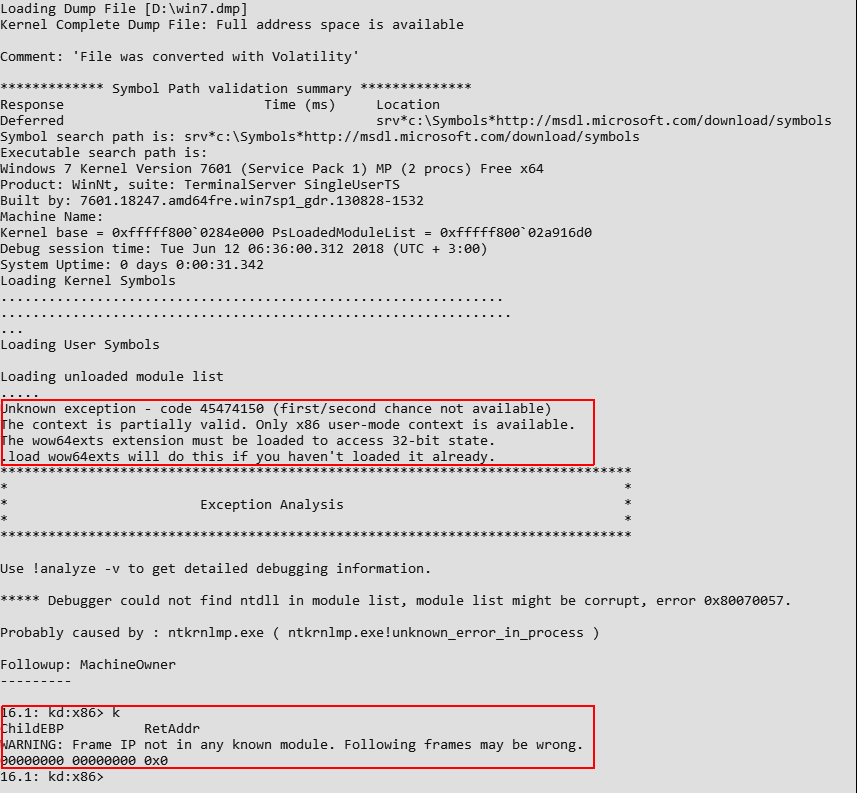
\includegraphics[width=1\textwidth]{vol1.png}
    \caption{WinDbg ошибочно интерпретирует отсутствующий контекст как 32-битный и не может отобразить стек вызовов на Windows 7}
    \label{fig:windbg-vol}
\end{center}
\end{figure}

\newpage
\section*{PVpanic и QEMU Guest Agent}

PVpanic -- виртуальное устройство на шине ISA, основным предназначением которого является генерация события в QEMU при аварийном завершении работы гостевой ОС.

QEMU Guest Agent -- специальная служба внутри гостевой ОС, которая помогает инструментам хоста управлять виртуальной машиной.

В 2017 году в драйвер PVpanic для Windows был добавлен ioctl-интерфейс, который позволяет пользовательскому приложению получать заголовок полного дампа памяти, с помощью вызова KeInitializeCrashDumpHeader (функция ядра Windows, сохраняющая заголовок полного дампа памяти, доступная драйверам\cite{kicdh}). По замыслу автора, этим приложением должен был быть QEMU Guest Agent. QEMU Guest Agent позволяет из хоста обращаться к файлам в гостевой ОС для записи и чтения, а для работы данного метода требовалось добавить возможность делать к файлам ioctl-запросы. Но сообщество разработчиков QEMU не приняло соответствующий патч, объяснив это тем, что добавляемая логика работы слишком сильно зависит от типа гостевой ОС.
Таким образом, этот метод так и остался не до конца реализованным.

\chapter{Описание метода}

Cобрать заголовок на хосте из содержимого памяти и регистров сложно по нескольким причинам:

\begin{itemize}
\item Неизвестно, где находится начало таблицы страниц для системного контекста. Для этого можно было бы использовать доступное гипервизору содержимое регистров CR3. Но возможна ситуация, при которой на всех виртуальных процессорах происходит исполнение пользовательских приложений, а в последних версиях современных ОС для x86 большая часть системной памяти не отображается в адресное пространство пользовательских процессов.
\item Поиск KdDebuggerDataBlock по сигнатуре затруднен, поскольку эта структура зашифрована в памяти новых версий Windows.
\item Поиск начала образа ядра Windows в памяти тоже нетривиален, поскольку при загрузке системы он принимает случайное значение благодаря технологии KASLR (англ. Kernel Address Space Layout Randomizing -- рандомизация размещения адресного пространства ядра), которая используется в новых версиях Windows.
\end{itemize}

Руководствуясь этими аргументами, а так же тем, что Windows предоставляет драйверам специальный интерфейс для получения заголовка дампа, решено разработать драйвер для гостевой системы, который получал бы заголовок и передавал его в гипервизор для дальнейшей обработки.

\section*{KeInitializeCrashDumpHeader}

KeInitializeCrashDumpHeader -- частично документированная функция, которая может быть вызвана драйвером для получения заголовка дампа.
В соответствии с официальной документацией, функция позволяет получить заголовок, который будет корректным всё время жизни системы, хотя и обладает следующими ограничениями:

\begin{itemize}
\item При изменении количества физической памяти заголовок должен быть получен снова
\item Полученный таким образом заголовок не содержит данных о возникшей ошибке (поле BugcheckData)
\end{itemize}

Также, согласно документации начиная с Windows 8, адрес таблицы страниц (DirectoryTableBase) в полученном заголовке всегда соответствует системному контексту, но для более ранних версий контекст будет совпадать с контекстом текущего процесса, в том числе может быть пользовательским, что затем может помешать отладчику осуществлять доступ к системным структурам по виртуальным адресам.

Кроме того, путем замены заголовка в сохраненном системой дампе (например после искусственно вызванного BSoD) на заголовок, полученный драйвером, и анализа такого модифицированного дампа обнаруживаются ещё несколько несоответствий:

\begin{itemize}
\item Не заполнено поле RequiredDumpSpace
\item Не заполнено поле Context (содержимое регистров одного из процессоров)
\item Поле PfnDatabase имеет неверное значение
\end{itemize}

Как уже было сказанно выше, структура KdDebuggerDataBlock содержит поля, дублирующие поля в заголовке, и это можно использовать для их исправления.
Способы восстановления полей заголовка собраны в соответствующей таблице:

\begin{table}[h]
\begin{tabular}{|c|c|c|}
\hline
Поле заголовка & Дамп на BSoD & Дамп живой системы \\
\hline
BugcheckData & \begin{minipage}{5.5cm}\begin{center}~\\Можно взять по адресу из поля KiBugcheckData внутри KdDebuggerDataBlock\\~\end{center}\end{minipage}& \begin{minipage}{5.5cm}\begin{center}~\\Использовать код 0x161 (LIVE{\_}SYSTEM{\_}DUMP)\\~\end{center}\end{minipage}\\
\hline
PfnDatabase &\multicolumn{2}{c|}{\begin{minipage}{11cm}\begin{center}~\\Можно взять из поля MmPfnDatabase внутри структуры KdDebuggerDataBlock\\~\end{center}\end{minipage}}\\
\hline
RequiredDumpSpace & \multicolumn{2}{c|}{\begin{minipage}{11cm}\begin{center}~\\Можно вычислить на основе информации о сохраненных регионах физической памяти\\~\end{center}\end{minipage}}\\
\hline
Context & \multicolumn{2}{c|}{\begin{minipage}{11cm}\begin{center}~\\Поле можно не заполнять, отладчик получает данные о значениях регистров каждого процессора из соответствующей ему структуры PRCB\\~\end{center}\end{minipage}}\\
\hline
\end{tabular}
\caption{Восстановление полей заголовка}
\end{table}

\section*{Транспорт для заголовка}

После того как заголовок получен, он должен быть передан в хост. Для этого можно использовать виртуальное устройство VMCoreInfo, которое изначально предназначено для передачи вспомогательных данных о ядре при создании дампов гостевой ОС Linux и является надстройкой над другим виртуальным аппаратным интерфейсом, называемым FwCfg. Обработка VMCoreInfo уже является частью функциональности создания дампов в формате ELF в QEMU, поэтому легко адаптируется для решаемой задачи. Также хорошим побочным эффектом является появление возможности создавать ELF-дампы, данных в которых потенциально достаточно их для конвертации в понятный WinDbg формат каким-либо внешним по отношению к QEMU инструментом.

\section*{FwCfg}

FwCfg -- виртуальный аппаратный интерфейс, предоставляемый QEMU, позволяющий гостевому ПО получать данные из хоста. С точки зрения гостевого ПО, представляет из себя устройство с портами ввода-вывода с номерами в диапазоне 0x510-0x51B. Предоставляет доступ к массиву записей (entry), которые могут быть как просто участками памяти, так и файлами на хостовой ОС. В зависимости от настроек, определяемых при создании каждой записи, может быть осуществлен доступ для чтения или модификации данных.

\section*{VMCoreInfo}

VMCoreInfo -- виртуальное устройство, доступ к которому осуществляется через одну из записей FwCfg. Изначально создано для добавления гостевой системой информации к дампам в ELF-формате, генерируемым QEMU.

\section*{Взаимодействие драйвера и VMCoreInfo}

Для того чтобы осуществлять запись или чтение из любой FwCfg-записи, в частности VMCoreInfo, драйвер использует порты ввода-вывода в диапазоне 0x510-0x51B.

Чтение данных из записи производится по следующему алгоритму:
\begin{enumerate}
\item В порт 0x510 отправляется номер записи, данные которой нужно прочитать
\item Из порта 0x511 побайтно считываются данные
\end{enumerate}

Чтобы записать данные в VMCoreInfo, нужно сначала эту найти запись по её названию (в данном случае -- "etc/vmcoreinfo"), а также проверить что в данной версии FwCfg возможна передача данных из гостя в хост:

\begin{enumerate}
\item Считывается запись номер 0x19 длиной 4 байта -- это суммарное количество записей
\item Считываются все записи и находится номер с подходящим названием
\item Проверяется значение восьми байт, считанных из портов 0x514--0x51B, они должны иметь значение 0x51454d5520434647 -- это означает, что поддерживается DMA-подобный интерфейс записи.
\end{enumerate}

В случае VMCoreInfo передается упакованная структура следующего вида:

\begin{verbatim}
struct FWCfgVMCoreInfo {
    uint16_t host_format;
    uint16_t guest_format;
    uint32_t size;
    uint64_t paddr;
} QEMU_PACKED;
\end{verbatim}

Поля host{\_}format и guest{\_}format должны быть равны соответственно 0 и 1, size -- размер передаваемых данных, paddr -- их физический адрес. 

Отправка данных осуществляется через DMA-подобный интерфейс:

\begin{enumerate}
\item В порты 0x514--0x51B записывается физический адрес структуры FWCfgDmaAccess, содержащей физический адрес записываемых данных, их длину, а также номер записи и управляющие биты.
\item Происходит проверка управляющих битов, если они все равны 0, то передача произошла успешно.
\end{enumerate}

После этого, QEMU будут доступны данные по адресу paddr. QEMU интерпретирует их как секцию ELF Note (рис. 3), которая состоит из названия (в данном случае "VMCOREINFO") и содержимого -- заголовка дампа\cite{elfspec}. Если структура секции корректна, то она становится доступна подсистеме создания дампов, и при создании ELF-дампа автоматически присоединяется к нему.

\begin{figure}[h]
\begin{center}
    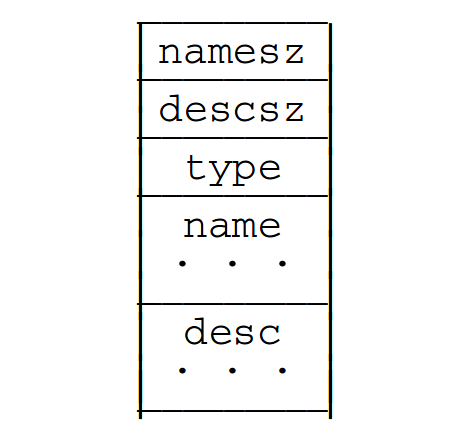
\includegraphics[width=5cm]{note.png}
    \caption{Структура секции ELF Note}
\end{center}
\end{figure}

Схема связи между структурами, участвующими в передаче заголовка показана на рисунке 4.

\begin{figure}[h]
\begin{center}
    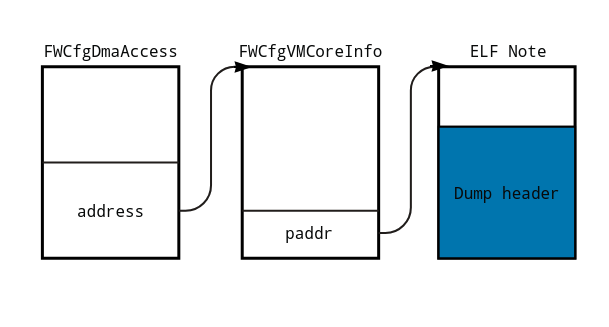
\includegraphics[width=1\textwidth]{vmci_scheme1.png}
    \caption{Упрощенная схема связи между структурами}
\end{center}
\end{figure}

\section*{Регистровый контекст}

В процессе отладки значения значения регистров важны сами по себе, но кроме того, их значения необходимы для корректного восстановления стека вызовов.

В файле wdm.h, который поставляется как часть WDK, есть определение структуры под названием CONTEXT. После сравнения этого определения, значений регистров из QEMU и поля Context из сохраненного Windows дампа, становится понятным, что поле Context содержит экpемпляр именно этой структуры. Но поскольку на современных системах количество процессоров больше одного, очевидно что регистровые контексты всех процессоров не могут поместиться в заголовке дампа (там выделено место ровно под один экземпляр контекста).

В структуре PRCB содержится поле ContextFrame. В сохраненном Windows полном дампе по адресу из этого поля содержится регистровый контекст процессора, которому соответсвует этот экземпляр структуры PRCB. Экспериментально выяснено, что WinDbg берет содержимое регистров именно из этих структур.

Поэтому, чтобы WinDbg cмог получить актуальные значения регистров, они должны быть сохранены в соответствующих структурах внутри дампа памяти. Независимая от версии Windows процедура может выглядеть так:

\begin{itemize}
\item Выяснение адресов PRCB всех процессоров из массива KdDebuggerDataBlock->KiProcessorBlock
\item Нахождение адресов контекстов по их смещению внутри PRCB\\на основе поля KdDebuggerDataBlock->OffsetPrcbContext
\item Заполнение контекстов, находящихся по этим адресам
\end{itemize}

\section*{Алгоритм работы компонента QEMU}

После того как заголовок доступен гипервизору, QEMU может приступать к созданию дампа.

\begin{enumerate}
    \item Виртуальная машина ставится на паузу.
    \item Производится синхронизация c KVM.
    \item Значение поля RequiredDumpSpace вычисляется как сумма размеров непрерывных регионов физической памяти, присутствующих в дампе, и подставляется в заголовок.
    \item Значение поля DirectoryTableBase из заголовка используются как значение регистра CR3 при дальнейшем доступе к виртуальному адресному пространству гостевой ОС из QEMU.
    \item Значения поля PfnDatabase подставляется из поля\newline KdDebuggerDataBlock->MmPfnDatabase.
    \item Значения полей BugcheckData (код и четыре параметра)
    \begin{itemize}
        \item Подставляются из полей KdDebuggerDataBlock->KiBugcheckData в случае дампа в момент аварийного завершения.
        \item Код 0x161 (LIVE{\_}SYSTEM{\_DUMP}), нулевые параметры в случае дампа живой системы.
    \end{itemize}
    \item Регистровый контекст сохраняется по адресу из поля KdDebuggerDataBlock->KiProcessorBlock[i]->ContextFrame, где i -- номер процессора, на основе регистров из QEMU (на этом этапе они уже имеют согласованное с KVM значение).
    \item Заголовок записывается в файл.
    \item Регионы физической памяти гостевой ОС на основе их описания в заголовке записываются в файл.
    \item Виртуальная машина может продолжать работу.
\end{enumerate}

\section*{KdDebuggerDataBlock в Windows 8 и более старших версиях}

Практика показывает, что начиная с Windows 8, KdDebuggerDataBlock может быть зашифрован системой на этапе ее загрузки и расшифровывается только во время аварийного завершения. Поэтому описанный выше метод будет работать в случае BSoD на любой из рассматриваемых версий Windows, но для снятия дампа с живой системы алгоритмы работы как драйвера, так и гипервизора должны быть дополнены с учетом этого факта. Поскольку метод основан на работе гостевого драйвера, то представляется наиболее простым получать расшифрованный KdDebuggerDataBlock так же с помощью драйвера.

\section*{KdDebuggerDataBlock и Small Memory Dump}

Наряду с полным дампом памяти, достаточно понятной является структура малого дамп памяти (Small Memory Dump). Windows создает дамп в этом формате после BSoD при настройках по умолчанию. Такой дамп содержит следующие данные:

\begin{itemize}
    \item Структура BugcheckData
    \item Данные о процессе, в котором возникла ошибка (структура EPROCESS)
    \item Информация о потоке, в котором возникла ошибка (структура ETHREAD)
    \item Контекст процессора (структура PRCB), на котором возникла ошибка
    \item Список загруженных модулей
    \item Структура KdDebuggerDataBlock
\end{itemize}

В отличие от полного дампа памяти, KdDebuggerDataBlock хранится в файле дампа по записанному в его заголовке смещению, поэтому страничное преобразвание не требуется. Таким образом, имея малый дамп, можно с его помощью создать полный дамп памяти.

\section*{KeCapturePersistentThreadState}

KeCapturePersistentThreadState -- недокументированная функция ядра Windows. Драйвер может использовать ее для сохранения в памяти Small Memory Dump. KdDebuggerDataBlock внутри такого дампа будет расшифрован.

Гостевой драйвер может передавать в гипервизор не только адрес оригинального KdDebuggerDataBlock (который может быть зашифрован), который система кладет в заголовок дампа, но и адрес его расшифрованной версии, которая будет храниться в памяти драйвера.

Для того чтобы гипервизор мог воспользоваться этой возможностью, он должен проверить сигнатуру KdDebuggerDataBlock, адрес которого лежит в своём обычном месте в заголовке, и, если сигнатура не совпадает, использовать KdDebuggerDataBlock, адрес которого может быть передан драйвером например через одно из неиспользуемых полей, например, BugcheckParameter1, поскольку это поле всё равно имеет нулевое значение и должно быть заполнено гипервизором.

Именно такой подход для передачи и обработки запасного KdDebuggerDataBlock и реализован в данной работе в гостевом драйвере и QEMU.

\chapter{Заключение}

В работе рассмотрено, какие данные требуются для создания полного дампа памяти ОС Windows. Для ОС Windows на основе ядра с номером 6.1 или старше представлен метод получения этих данных, который не зависит от конкретной версии Windows и, возможно, будет работать и с появлением новых версий. Также разработан метод передачи необходимой информации в гипервизор.

Реализован драйвер, непосредственно собирающий необходимую для создания дампа информацию из гостевой системы. Код драйвера опубликован как часть проекта KVM Windows Guest Drivers.
Разработан патч для QEMU, добавляющий команде dump-guest-memory новый ключ '-w', который позволяет напрямую, без конвертации, создавать дампы в формате DMP (может быть проанализирован WinDbg или kd.exe), если внутри гостевой системы работает драйвер. Кроме того, дампы в формате ELF также будут содержать всю необходимую для дальнейшей конвертации в формат DMP информацию.

\chapter{Возможные направления дальнейшего развития проекта}

Вариантами возможного продолжения данной работы являются следующие направления:
\begin{itemize}
\item Поскольку одним из вариантов использования технологии виртуализации является отказ от устаревшей аппаратной платформы и перенос ПО в соответствующую виртуализованную среду, следует рассмотреть добавление возможности работы представленного механизма с 32-разрядными версиями Windows.
\item Существует способ динамического увеличения размера доступной виртуальной машине памяти под названием RAM hot-plug, который заключается в динамическом добавлении виртуальных модулей памяти. В настоящее время драйвер не создает новый заголовок в такой ситуации, но возможно сделать обработку этого случая с помощью стандартных событий.
\item Одним из наиболее популярных гипервизоров для запуска виртуальных машин с операционной системой Windows является проприентарный гипервизор Hyper-V от корпорации Microsoft.\\Для того чтобы сделать дамп памяти гостевой Windows, работающей под Microsoft Hyper-V, можно использовать одну из утилит Sysinternals Suite -- LiveKd\cite{livekd-hv}. Эта программа позволяет по идентификатору виртуальной машины, работающей под управлением Hyper-V, сделать полный дамп памяти этой виртуальной машины и сохранить его на файловой системе хостовой операционной системы. Примечательно, что для работы этого механизма не требуется делать никаких настроек внутри виртуальной машины, в том числе не требуется устанавливать дополнительные драйверы.\\Таким образом, одним из возможных направлений дальнейшей работы является подробное исследование работы этого инструмента и попытка реализовать аналогичный механизм как компонент QEMU/KVM.
\newpage
\item В рассмотреной в работе схеме заголовок полного дампа памяти может быть получен как одна из секций дампа в формате ELF. На данный момент, такие утилиты как Volatility при попытке конвертации дампа из ELF формата не используют данные VMCOREINFO. Возможно добавить такой сценарий работы в Volatility, что позволило бы Volatility правильно производить конвертацию.
\end{itemize}

\printbibliography

\end{document}
